\part{Metodologia}

\chapter[Metodologia]{Metodologia}

\section{Definição do processo}

\begin{figure}[ht]
	\centering
	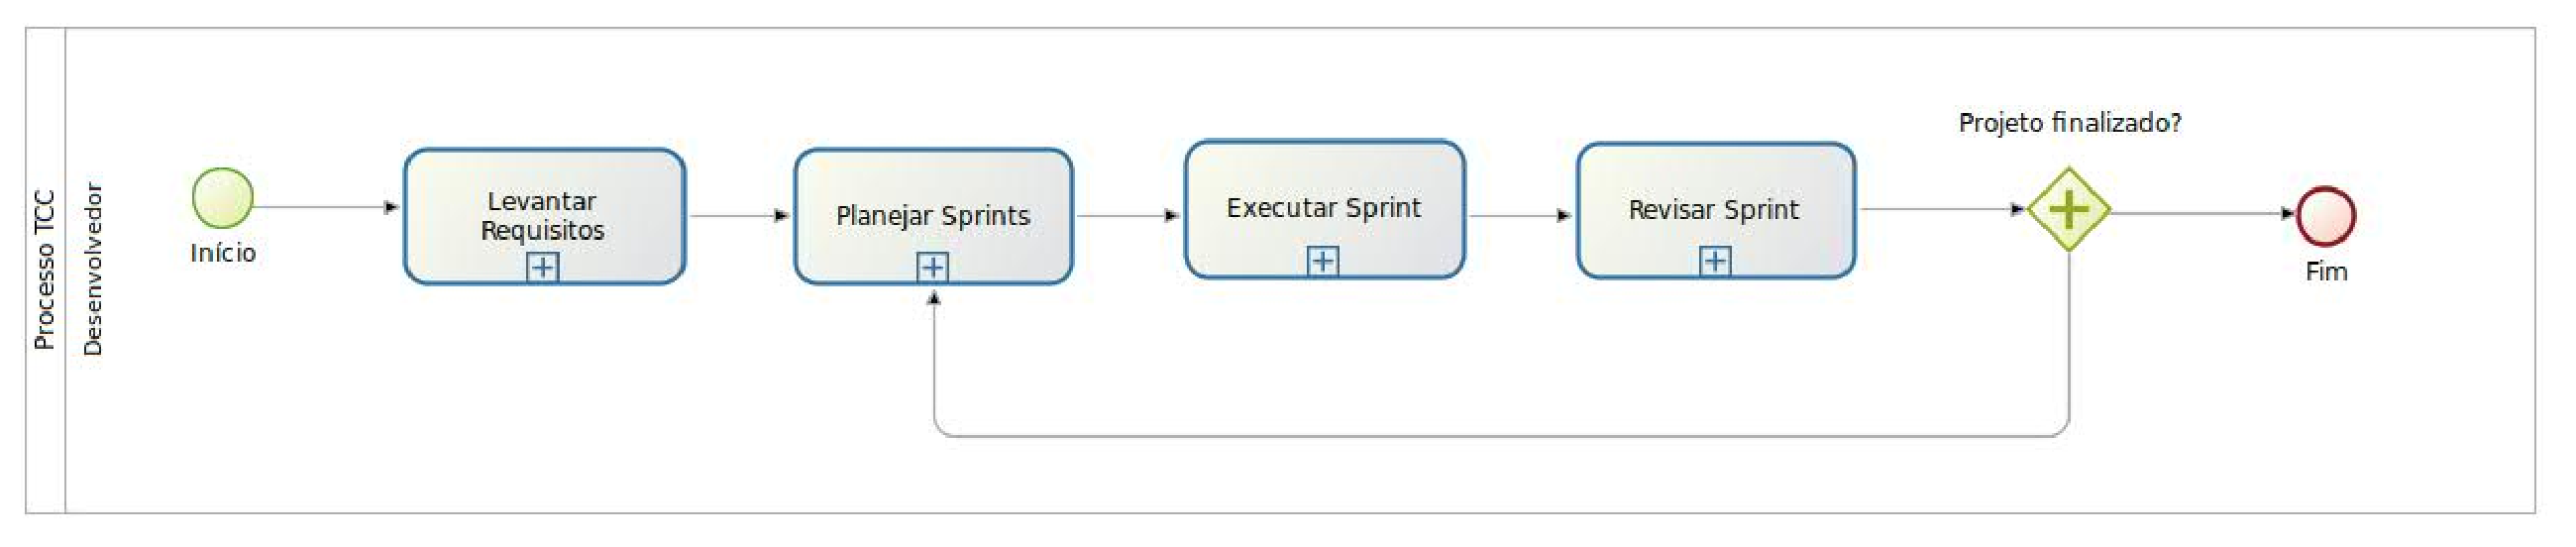
\includegraphics[keepaspectratio=true,scale=0.9, width=\textwidth]{figuras/fig06.eps}
	\caption{Práticas do XP \cite{Beck:2004}}
	\label{fig06}
\end{figure}

\begin{figure}[ht]
	\centering
	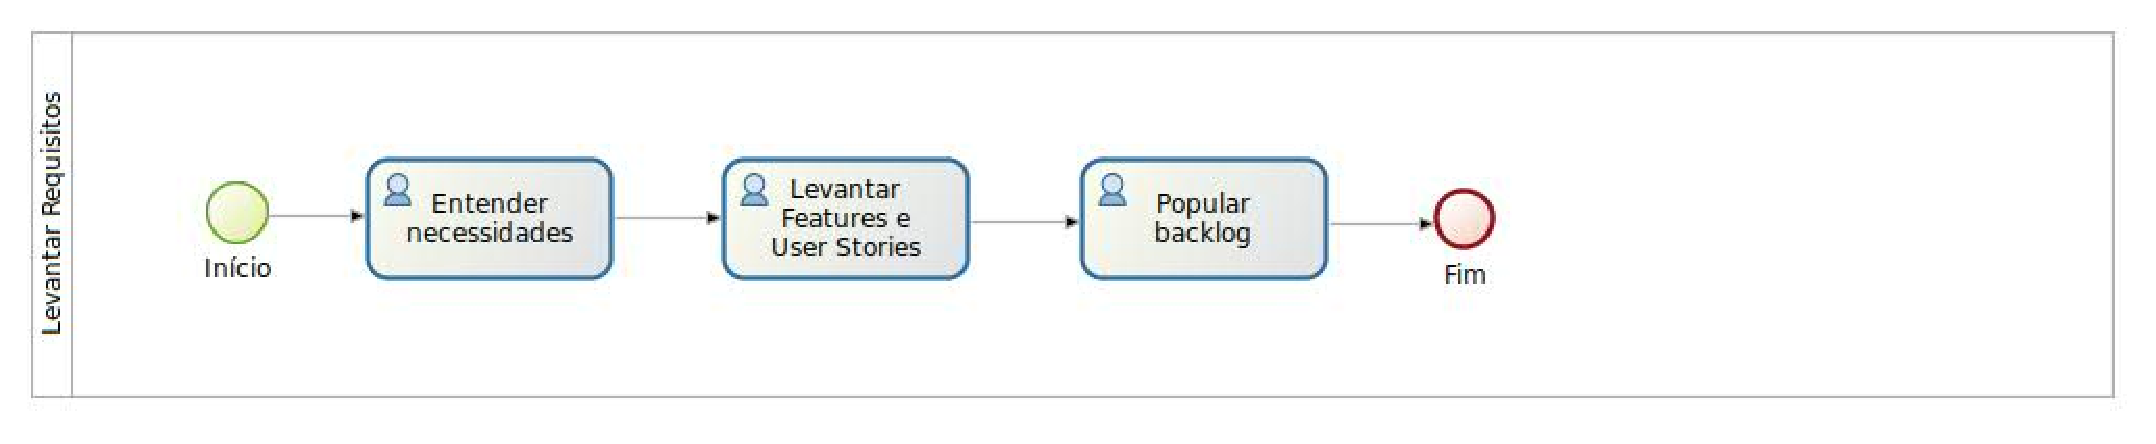
\includegraphics[keepaspectratio=true,scale=0.9, width=\textwidth]{figuras/fig07.eps}
	\caption{Práticas do XP \cite{Beck:2004}}
	\label{fig07}
\end{figure}

\begin{figure}[ht]
	\centering
	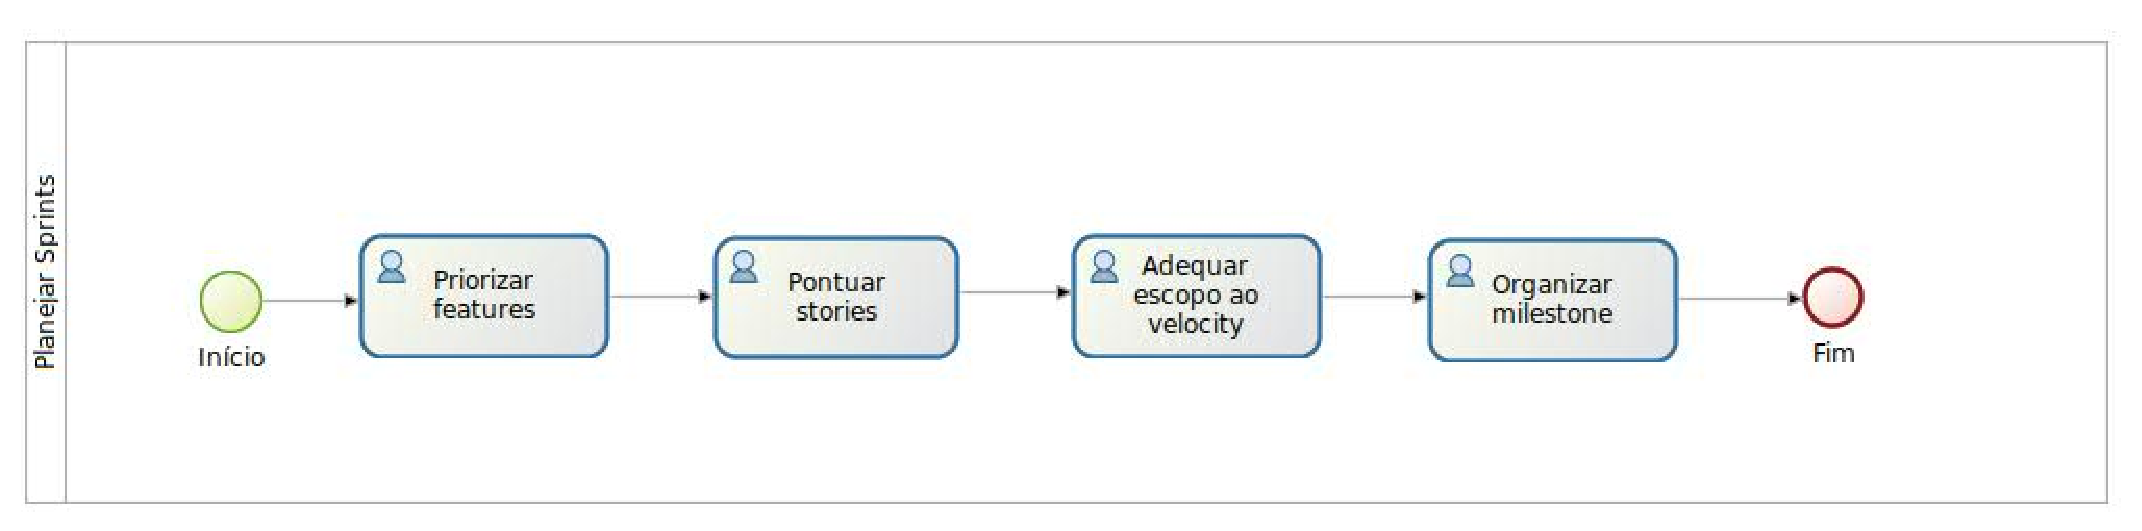
\includegraphics[keepaspectratio=true,scale=0.9, width=\textwidth]{figuras/fig08.eps}
	\caption{Práticas do XP \cite{Beck:2004}}
	\label{fig08}
\end{figure}

\begin{figure}[ht]
	\centering
	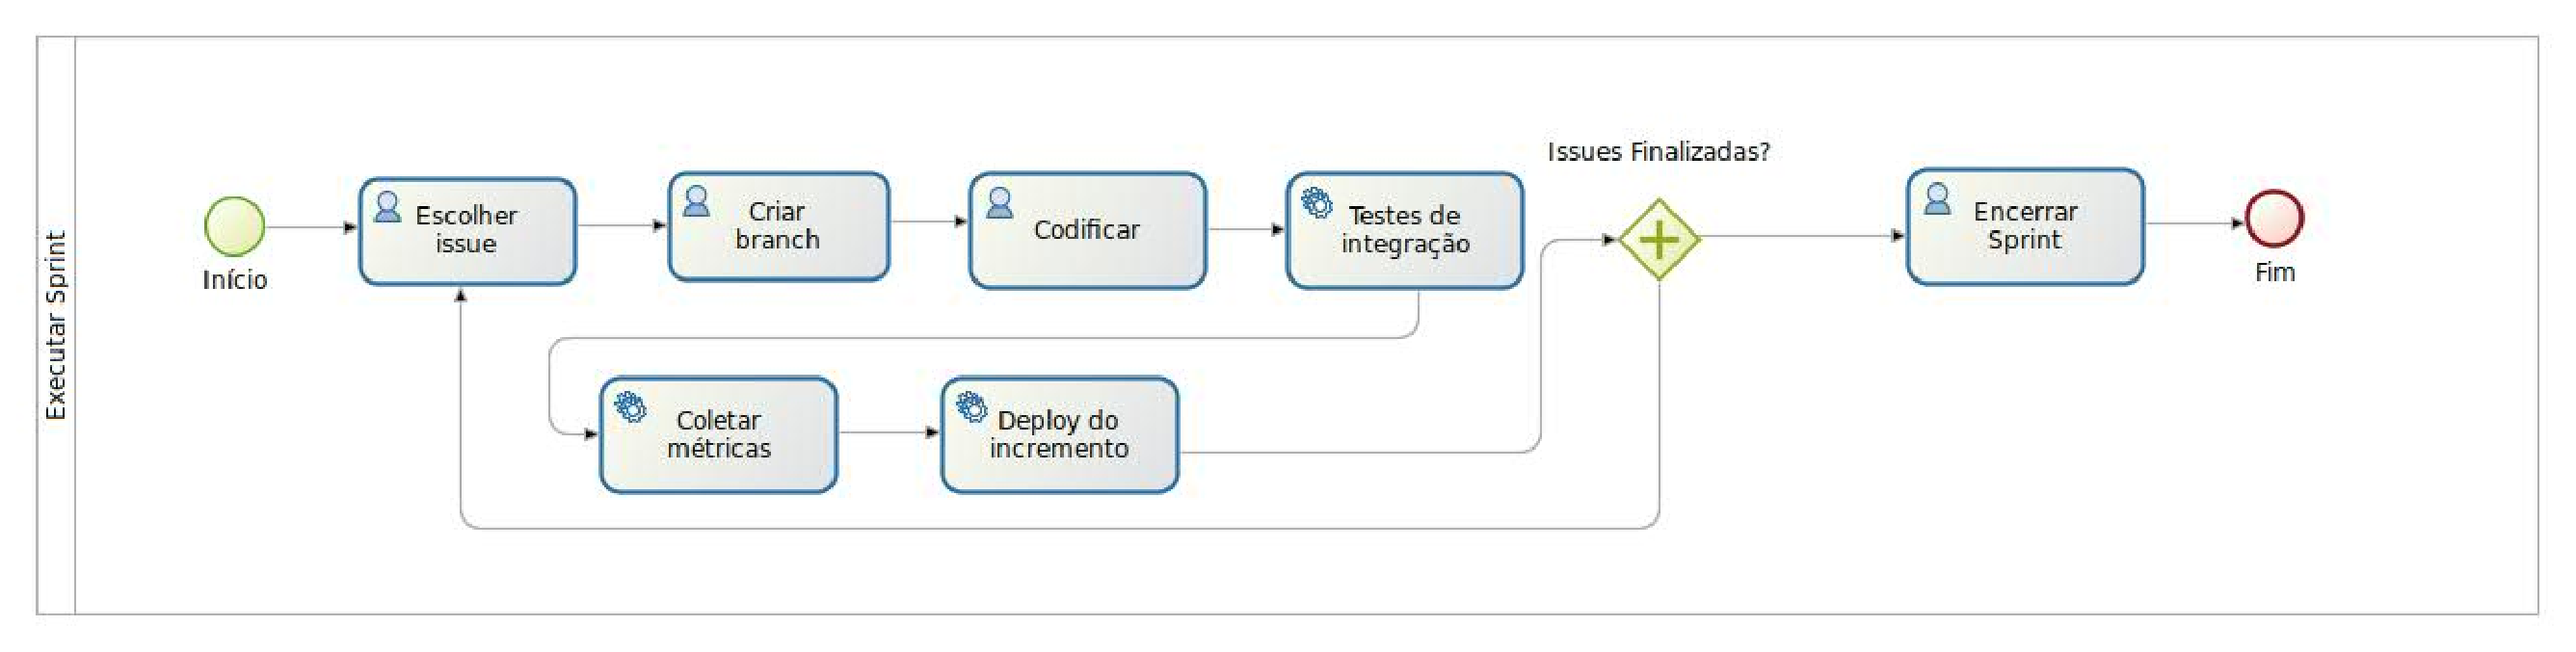
\includegraphics[keepaspectratio=true,scale=0.9, width=\textwidth]{figuras/fig09.eps}
	\caption{Práticas do XP \cite{Beck:2004}}
	\label{fig09}
\end{figure}

\begin{figure}[ht]
	\centering
	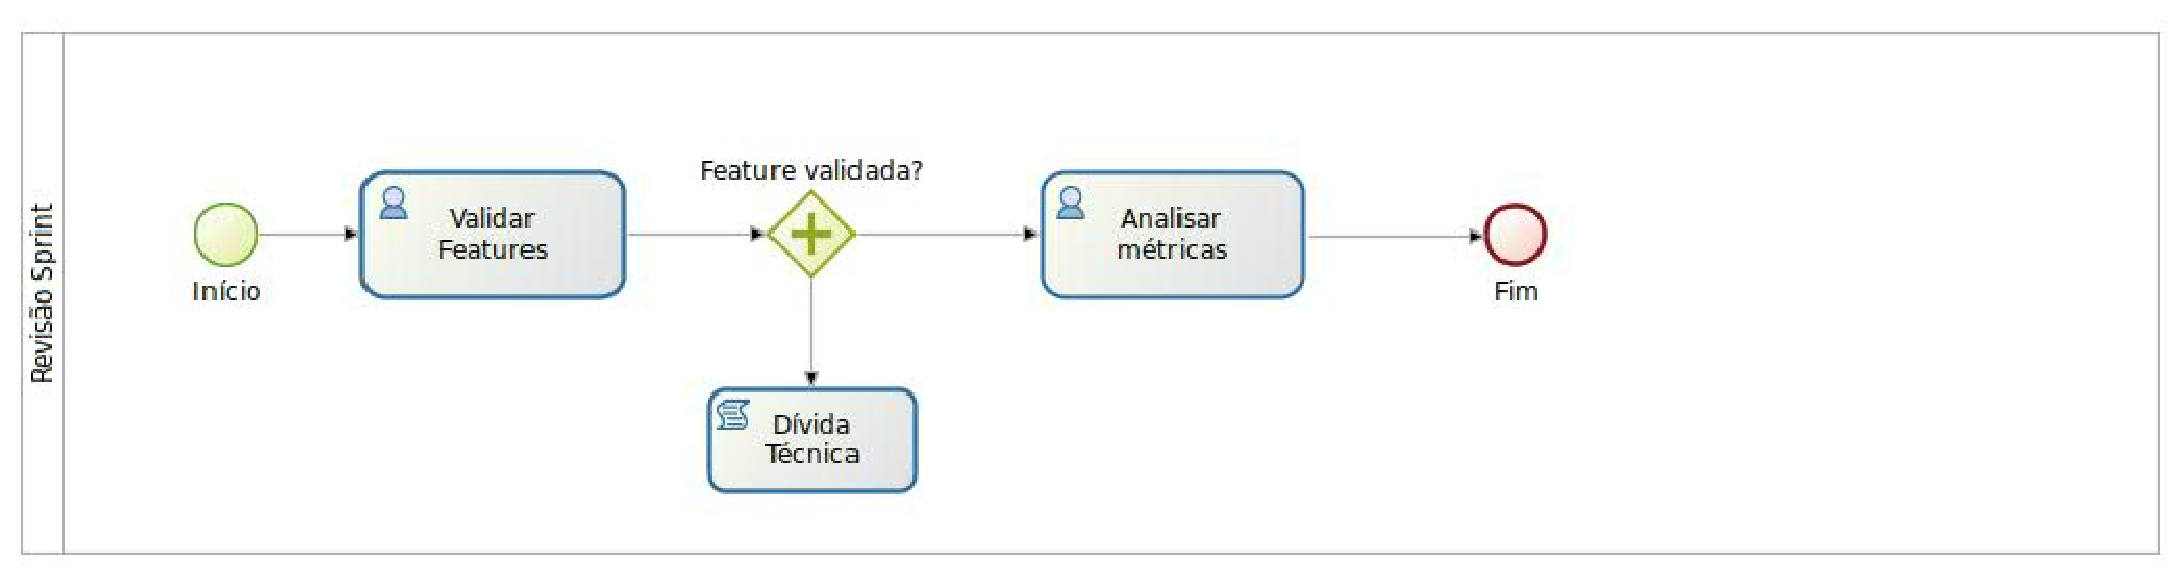
\includegraphics[keepaspectratio=true,scale=0.9, width=\textwidth]{figuras/fig10.eps}
	\caption{Práticas do XP \cite{Beck:2004}}
	\label{fig10}
\end{figure}
